\chapter{Recursos: como criar e configurar}

\section{Conteúdo do pacote IMS}

IMS Global Learning Consortium, ou simplesmente IMS, refere-se a um consórcio entre instituições de ensino, editoras, empresas do setor tecnológico, organizações governamentais e iniciativas regionais que se organizaram com intuito de apoiar o uso da tecnologia como forma de transformar a aprendizagem educacional (CONSORTIUM, 2011).

Um pacote IMS refere-se a uma estrutura de arquivos criados sob as especificações do padrão \emph{IMS Content Packaging}. Pacotes IMS permitem a exportação e importação de conteúdo de um ambiente virtual de aprendizado para outro, indicando seu reaproveitamento (SPECIFICATION, 2011).

Muitos softwares permitem a exportação de seu conteúdo por meio de pacotes IMS, entre eles pode-se citar o
ExeLearning (\url{http://exelearning.org}) e o Reload (\url{http://www.reload.ac.uk}).

Apesar de sua grande utilidade e funcionalidade, este recurso ainda é pouco explorado devido a alguns problemas ocorridos no reaproveitamento de conteúdo entre versões distintas de ambientes virtuais de aprendizagem (SILVA, 2010). 

\subsection{Acrescentando o recurso Conteúdo do pacote IMS}

Para acrescentar o recurso Conteúdo do pacote IMS deve-se:
\begin{enumerate}
\item Na disciplina desejada, clicar no botão \textbf{Ativar edição};
\item Primeiro deve-se clicar na opção \textbf{Adicionar uma atividade ou recurso}, e só então aparecerá a opção de \textbf{Acrescentar}. Em seguida, basta escolher a opção \textbf{Conteúdo od pacote IMS} na lista \textbf{Recursos} e clicar em \textbf{Acrescentar};
\item No formulário apresentado, preencher obrigatoriamente os campos \textbf{Nome} (nome do recurso que ficará visível na plataforma) e \textbf{Descrição} (informações gerais sobre o recurso);
\item Clicar no botão  \textbf{Escolher um arquivo}  selecionar o pacote IMS e enviá-lo.
\end{enumerate}

Alguns softwares oferecem a possibilidade de unir vários pacotes IMS em apenas um. Se esse for o caso, na opção \textbf{Arquivos de pacote}, selecionar a quantidade de pacotes que foram unidos;

Na opção \textbf{Visível}, informar se o recurso ficará disponível ou oculto para os alunos;
caso necessário, preencher o campo \textbf{Número de identificação do módulo} para fins de cálculo de avaliação.

Salvar as configurações realizadas clicando no botão \textbf{Salvar e voltar ao curso}  para salvar e retornar para a disciplina ou no botão \textbf{Salvar e mostrar }para salvar e mostrar o recurso criado.

\section{Página}

O Recurso página, illutrada na Figura \ref{fig:cap4_1}, é um recurso muito utilizado no Moodle, pois possui inúmeras finalidades. Ela pode ser utilizada para disponibilizar avisos, ementas, cronogramas, horários, álbum de fotos, videoteca, lista de links, lista de endereços de contato, entre outras possibilidades. Além disso, o recurso página segue os mesmos princípios de edição do \textit{HyperText Markup Language }(HTML).
\begin{figure}[htbp]
 \begin{center}
 \fbox{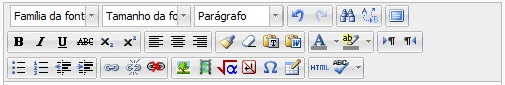
\includegraphics[width=0.6\textwidth]{imagem/cap4/fig1.jpg}}
  \caption{Página}
  \label{fig:cap4_1}
 \end{center}
\end{figure}
A semelhança com o editor de texto Word da Microsoft\footnote{Empresa multinacional de tecnologia e informática} também facilita a construção deste recurso. A seguir apresenta-se o menu de formatação e edição de textos do Moodle.

Este menu é comum a diversos recursos e atividades, suas opções são listadas na Tabela \ref{table:cap4_table1}.

\begin{table}[htbp]
\begin{flushleft}
\begin{tabular}{p{8cm}|p{6cm}} \hline
\rowcolor[rgb]{0.8,0.8,0.8} \textbf{Ícone}& \textbf{Descrição}\\\hline
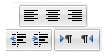
\includegraphics[width=0.1\textwidth]{imagem/cap4/fig2.jpg} & Alinhamento e posicionamento do texto \\\hline
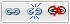
\includegraphics[width=0.07\textwidth]{imagem/cap4/fig3.jpg} & Inserção, remoção e impedimento de links \\\hline
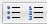
\includegraphics[width=0.08\textwidth]{imagem/cap4/fig4.jpg} & Marcadores e numeração \\\hline
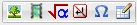
\includegraphics[width=0.15\textwidth]{imagem/cap4/fig5.jpg} & Inserção de imagem, vídeo, equação, caracteres especiais, espaço em branco e tabela\\\hline

\includegraphics[width=0.09\textwidth]{imagem/cap4/fig6.jpg} & Definição de cores\\\hline
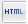
\includegraphics[width=0.09\textwidth]{imagem/cap4/fig7.jpg} & Editor de linguagem HTML\\\hline
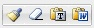
\includegraphics[width=0.13\textwidth]{imagem/cap4/fig8.jpg} & Remoção de código incorreto e formatação, colagem de textos\\\hline
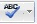
\includegraphics[width=0.08\textwidth]{imagem/cap4/fig9.jpg} & Corretor ortográfico\\\hline
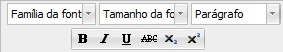
\includegraphics[width=0.25\textwidth]{imagem/cap4/fig10.jpg} & Definição do tipo e tamanho da fonte, parágrafo e outras características gerais do texto\\\hline
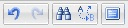
\includegraphics[width=0.25\textwidth]{imagem/cap4/fig11.jpg} & Desfazer (CTRL+Z), refazer (CTRL+Y), localizar/substituir, tela inteira.\\\hline
\end{tabular}
\caption{Configurações de Página}
  \label{table:cap4_table1}
\end{flushleft}
\end{table}%

Aconselha-se que cada funcionalidade do editor de texto seja testada pelo usuário, já que a manipulação correta dos recursos do editor pode facilitar e agilizar a construção de um texto. A função de cada item do editor é exibida toda a vez que se posiciona o ponteiro do mouse sobre cada ícone.

\subsection{Acrescentando o recurso página}

Para acrescentar o recurso Página deve-se seguir os passos abaixo:
\begin{enumerate}
\item Na disciplina desejada, clicar no botão \textbf{ Ativar edição};
\item Primeiro deve-se clicar na opção \textbf{Adicionar uma atividade ou recurso}, e só então aparecerá a opção de \textbf{Acrescentar}. Em seguida basta escolher a opção \textbf{Página} na lista \textbf{Recursos} e clicar em \textbf{Acrescentar};
\item No formulário apresentado, preencher obrigatoriamente os campos \textbf{Nome} (nome do recurso que ficará visível na plataforma) e \textbf{Descrição} (informações gerais sobre o recurso);
\item O campo \textbf{conteúdo da página}, como o próprio nome sugere, é responsável por aquilo que será exibido para o usuário. Este campo também é de preenchimento obrigatório;
\item Caso seja necessário, marcar a caixa de seleção \textbf{mostrar o nome da página}. Ela é responsável por exibir o nome da página após o clique do usuário no recurso página;
\item Caso seja necessário, marcar a caixa de seleção \textbf{exibir descrição da página}. Ela é responsável por exibir o conteúdo preenchido no campo descrição da página, após o clique do usuário neste recurso;
\item Na opção \textbf{Visível}, informar se o recurso ficará disponível ou oculto para os alunos;
\item Caso seja necessário, preencher o campo \textbf{Número de identificação do módulo} para fins de cálculo de avaliação.
\item Salvar as configurações realizadas clicando no botão  \textbf{Salvar e voltar ao curso} para salvar e retornar para a disciplina ou no botão \textbf{Salvar e mostrar } para salvar e exibir a página criada.
\end{enumerate}

\subsection{Inserindo uma imagem em uma página}

Para inserir uma imagem em uma página, deve-se clicar no ícone: 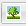
\includegraphics{imagem/cap4/fig12.jpg}. Uma janela, como aquela illustrada na Figura \ref{fig:cap4_13}, será exibida. Basta então clicar em \textbf{Encontrar} ou enviar uma imagem para poder selecionar a imagem que se deseja
adcionar a uma página.

\begin{figure}[htbp]
 \begin{center}
 \fbox{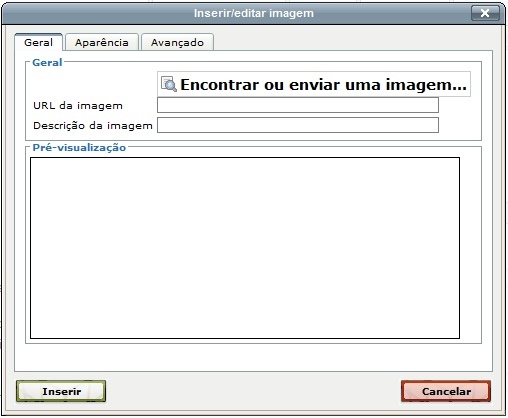
\includegraphics[width=0.5\textwidth]{imagem/cap4/fig13.jpg}}
  \caption{Enviando Imagem}
  \label{fig:cap4_13}
 \end{center}
\end{figure}

Na próxima janela exibida (Figura \ref{fig:cap4_14}), clicar em \textbf{Enviar um arquivo} e em seguida em \textbf{Escolher um arquivo}.
\begin{figure}[htbp]
 \begin{center}
 \fbox{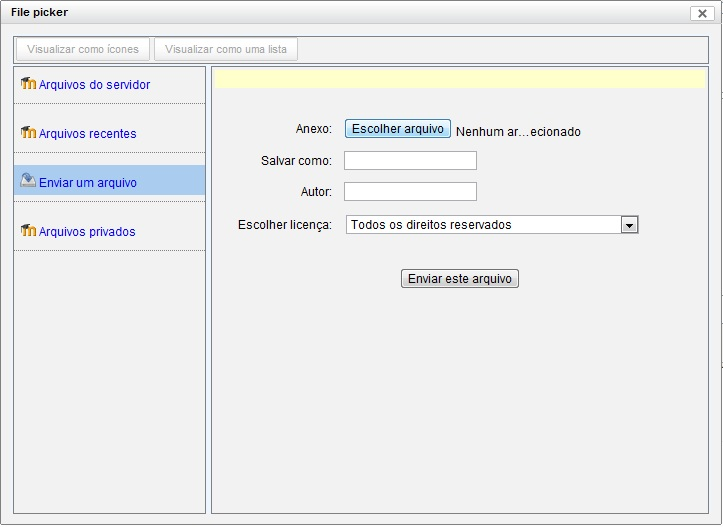
\includegraphics[width=0.5\textwidth]{imagem/cap4/fig14.jpg}}
  \caption{Enviando Arquivo}
  \label{fig:cap4_14}
 \end{center}
\end{figure}
Selecionar em seu computador a imagem que deseja inserir.

Clicar em \textbf{Enviar este arquivo} (a janela anterior se fechará e retornará primeira janela).

Na janela exibida, informar uma descrição para a imagem enviada e clicar em \textbf{Inserir} para incluir a imagem na página.

Com a imagem já inserida na página, pode-se organizar sua posição e tamanho com o auxílio das ferramentas de edição.

\subsection{Inserindo vídeo em uma página}

O YouTube (\url{http://www.youtube.com}) é uma boa fonte de vídeos, permitindo que seus usuários compartilhem vídeos em formato digital.
Para inserir um vídeo do YouTube em uma página, deve-se seguir os passos abaixo:

\begin{enumerate}
\item Acessar o sítio do YouTube e localizar o vídeo que deseja inserir;

\item Ainda no sítio do YouTube, abaixo do vídeo desejado, clicar no botão \textbf{Compartilhar} e em seguida no botão \textbf{Incorporar};

\item Selecionar e copiar (CTRL+C) o código que for exibido na caixa de seleção, conforme Figura abaixo:

 \begin{center}
 \fbox{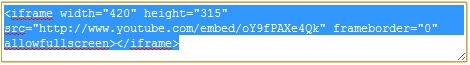
\includegraphics[width=0.7\textwidth]{imagem/cap4/fig15.jpg}}
 \end{center}

\item Retornar para o Moodle e criar o recurso página;
\item No campo \textbf{Descrição}, mover o cursor\footnote{Indicador usado para indicar a posição que irá responder à adição de texto ou movimentos do mouse}  na posição desejada para inserir o vídeo e clicar no ícone \textbf{HTML};
\item Na janela exibida, colar o código copiado na posição desejada. Na linguagem HTML, os indicadores <p></p> correspondem a um parágrafo, neste sentido, aconselha-se inserir o código entre esses dois indicadores, por exemplo, <p>\textbf{CÓDIGO COPIADO}</p>, conforme a Figura abaixo:

 \begin{center}
 \fbox{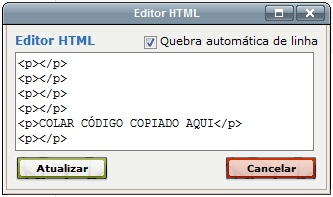
\includegraphics[width=0.4\textwidth]{imagem/cap4/fig16.jpg}} 
 \end{center}

\item Clicar no botão \textbf{Atualizar} e em seguida salvar a página.
\end{enumerate}

\section{Pasta}

A \textbf{pasta}, assim como a \textbf{página}, também é um recurso bastante utilizado no Moodle. Ele é útil para reunir e disponibilizar os arquivos de maneira organizada na disciplina, evitando que a área central fique poluída e minimizando possíveis dúvidas por parte dos alunos em relação à divisão de conteúdo.

O recurso \textbf{pasta} no Moodle é análogo ao esquema de diretórios de um computador. É possível criar uma infinidade de diretórios, onde cada diretório pode armazenar vários arquivos ou até mesmo outros diretórios. Na estrutura mostrada na Figura \ref{fig:cap4_17}, é apresentado um esquema onde o diretório chamado \textbf{Semestre1} armazena outro diretório de nome \textbf{Estágio1} e um arquivo chamado \textbf{Cores.png}. O diretório\textbf{ Estágio1}, por sua vez, possui o arquivo \textbf{roteiro.txt} disponível em seu interior.

\begin{figure}[htbp]
 \begin{center}
 \fbox{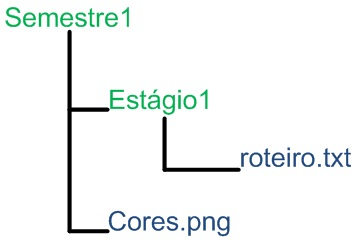
\includegraphics[width=0.4\textwidth]{imagem/cap4/fig17.jpg}}
  \caption{Representação}
  \label{fig:cap4_17}
 \end{center}
\end{figure}

\subsection{Acrescentando o recurso pasta}
Para criar o recurso \textbf{pasta}, deve-se:

\begin{enumerate}
\item Na disciplina desejada, clicar no botão 
\includegraphics[width=0.1\textwidth]{imagem/cap4/fig18.jpg} ;
\item Primeiro deve-se clicar na opção \textbf{Adicionar uma atividade ou recurso}, e só então aparecerá a opção \textbf{Acrescentar}. Em seguida basta escolher a opção \textbf{Pasta} na lista \textbf{Recursos} e clicar em \textbf{Acrescentar};

     \begin{center}
     \fbox{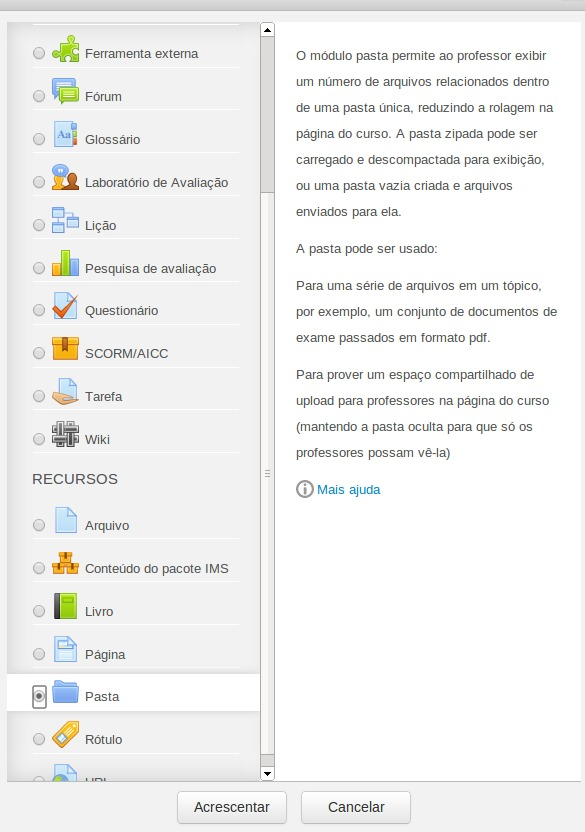
\includegraphics[width=0.4\textwidth]{imagem/cap4/fig19.jpg}}
     \end{center}

\item No formulário apresentado, preencher obrigatoriamente os campos \textbf{Nome} (nome da pasta que ficará visível na plataforma) e \textbf{Descrição} (informações gerais sobre o recurso);
\item Clicar no botão \textbf{Criar Diretório}  para adicionar um novo diretório;
\item Na janela exibida, informar o nome da pasta, conforme a Figura a seguir;

         \begin{center}
         \fbox{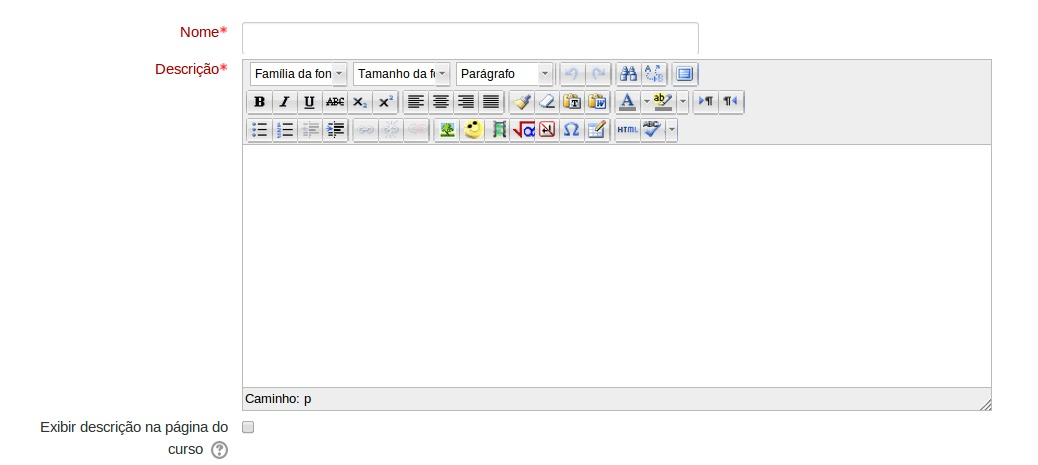
\includegraphics[width=0.5\textwidth]{imagem/cap4/fig20.jpg}}
         \end{center}
\item Na opção \textbf{Visível}, informar se o recurso ficará disponível ou oculto para os alunos. Caso necessário, preencher o campo\textbf{ Número de identificação }do módulo para fins de cálculo de avaliação;
\item Salvar as configurações realizadas clicando no botão \textbf{Salvar e voltar ao curso } para salvar e retornar para a disciplina ou no botão \textbf{Salvar e mostrar } para salvar e mostrar o recurso criado.
\end{enumerate}


\subsection{Enviando arquivo para uma pasta}
Para enviar um arquivo para uma pasta já criada, deve-se:
\begin{enumerate}
\item Ir até a disciplina desejada e clicar na pasta onde se deseja inserir o arquivo. Clicar no botão \textbf{Editar};
\item Se necessário, clicar sobre o nome do diretório em que se deseja inserir o arquivo;
\item Observar o \textbf{tamanho máximo para novos arquivos}. Este parâmetro limita o tamanho do arquivo a ser enviado para o ambiente. Este limite pode variar de plataforma para plataforma. Sua configuração é determinada tanto pelo administrador do Moodle como pelo professor da disciplina.
\item Clicar no botão \textbf{Adicionar};
\item Na próxima janela exibida, clicar em \textbf{Enviar um arquivo} e em seguida em \textbf{Escolher um arquivo} (Veja a Figura \ref{fig:cap4_14});
\item Selecionar em seu computador o arquivo que deseja inserir na pasta;
\item Clicar em \textbf{Enviar este arquivo} (a janela anterior se fechará e retornará a tela anterior);
\item Por fim, clicar no botão \textbf{Enviar}.

\end{enumerate}
É possível \textbf{criar um diretório dentro de outro diretório}, para isso basta seguir os passos anteriores e, antes clicar no botão \textbf{Adicionar}, clicar em \textbf{Criar Diretório} e, em seguida, informar o nome do diretório desejado.

Desta maneira é possível criar uma estrutura de pastas semelhante a do seu computador, com vários níveis de organização. É importante ressaltar que a criação excessiva de níveis de diretórios pode confundir os alunos e deve ser evitada.

\subsection{Organizando os arquivos da disciplina}
Organizar os arquivos da disciplina é fundamental. Arquivos desagrupados podem confundir e desorientar os alunos.
Esta sessão tem o objetivo de, com os arquivos já inseridos, orientar o ministrante do curso sobre as maneiras de 
organizar seus arquivos, movendo e excluindo o conteúdo da disciplina.

\subsection{Excluindo arquivos ou diretórios}

Para excluir arquivos ou diretórios, deve-se:

\begin{enumerate}
\item Ir até a disciplina desejada e clicar na pasta onde se deseja excluir o arquivo ou diretório;
\item Clicar no botão \textbf{Editar};
\item Dentro da pasta, localizar o diretório ou arquivo que deseja excluir;
\item Clica-se no arquivo desejado;
\item Aparecerá outro menu com opção com os ítens: \textbf{Excluir}, \textbf{Renomear}, entre outros;
\item Em qualquer dos menus, clicar no item \textbf{Excluir};
\item Na janela exibida, clicar no botão \textbf{Ok};
\item Para confirmar a exclusão ainda é necessário clicar no botão \textbf{Salvar Mudanças}.
\end{enumerate}
É importante ressaltar que para concluir o procedimento de exclusão a realização do último passo é imprescindível. Caso isso não aconteça, as modificações realizadas não serão salvas, em outras palavras, o arquivo ou diretório não será excluído.

Outro ponto importante é que a exclusão de um diretório implica na exclusão dos arquivos que estão em seu interior.

\subsection{Movendo arquivos ou diretórios}
Para mover arquivos ou diretórios, deve-se:
\begin{enumerate}
\item Ir até a disciplina desejada e clicar na pasta onde se deseja mover o arquivo;
\item Clicar no botão \textbf{Editar};
\item Dentro da pasta, localizar o diretório ou arquivo que deseja mover;
\item Clica-se no diretório desejado;
\item Aparecerá outro menu com opção com os ítens: \textbf{Excluir}, \textbf{Renomear}, entre outros;
\item Em qualquer dos menus, clicar no item \textbf{Mover};
\item Na janela exibida, clicar no botão \textbf{Ok};
\item Para confirmar a modificação ainda é necessário clicar no botão \textbf{Enviar}.
\end{enumerate}
É importante ressaltar que para concluir o procedimento de mover um arquivo ou diretório, a realização do último passo é imprescindível. Caso isso não aconteça, as modificações realizadas não serão salvas, em outras palavras, o arquivo ou diretório não será movido.

\subsection{Renomeando arquivos ou diretórios}
Para renomear arquivos ou diretórios deve-se:
\begin{enumerate}
\item Ir até a disciplina desejada e clicar na pasta onde se deseja renomear o arquivo ou diretório;
\item Clicar no botão \textbf{Editar};
\item Dentro da pasta, localizar o diretório ou arquivo que deseja renomear;
\item Clicar no ícone quando for diretório, ou sobre o arquivo;
\item Dependendo do item, o menu exibido pode ser de duas formas;
\item Em qualquer dos menus, clicar no item \textbf{Atualizar};
\item Na janela exibida, informar o novo nome para o arquivo ou diretório e clicar no botão \textbf{Ok};
\item Para confirmar, ainda é necessário clicar no botão \textbf{Salvar Mudanças}.
\end{enumerate} 
É importante ressaltar que para concluir o procedimento de renomear um arquivo ou diretório, a realização do último passo é imprescindível. Caso isso não aconteça, as modificações realizadas não serão salvas, em outras palavras, o arquivo ou diretório não será renomeado.

Outro ponto importante é que ao se alterar o nome de um arquivo deve-se preservar a sua extensão.\footnote{Extensão de um arquivo refere-se ao tipo. Por exemplo, arquivos de imagem podem ter extensão jpg ou png. Arquivos de texto podem ter extensão doc, docx, txt ou rtf.} Caso isto não aconteça, o tipo do arquivo pode ser modificado, ocasionando problemas quando o aluno tentar abrir o arquivo em seu computador.


\subsection{Compactando e descompactando arquivos e diretórios}
Para compactar diretórios, deve-se:

\begin{enumerate}
\item Ir até a disciplina desejada e clicar na pasta onde se deseja compactar o diretório;
\item Clicar no botão \textbf{Editar};
\item Dentro da pasta, localizar o diretório que deseja compactar;
\item Clicar no ícone 
\includegraphics{imagem/cap4/fig21.jpg} e em seguida opção \textbf{Zip};
\item Para confirmar a compactação ainda é necessário clicar no botão \textbf{Salvar mudanças}. Será criado um arquivo compactado com a extensão .zip com o mesmo nome do diretório original. Vale salientar que o diretório original não é apagado, mas será mantido juntamente com o arquivo compactado.
\end{enumerate}
Para descompactar arquivos ou diretórios, deve-se:
\begin{enumerate}
\item Ir até a disciplina desejada e clicar na pasta onde se deseja descompactar o arquivo ou diretório;
\item Clicar no botão \textbf{Editar};
\item Dentro da pasta, localizar o arquivo que deseja descompactar;
\item Clicar sobre o arquivo e em seguida na opção \textbf{Descompactar};
\item No caso da descompactação de diretórios, será criado um diretório com o nome 0 (zero) com os arquivos contidos dentro do diretório compactado. Caso já exista uma pasta com o nome 0, os arquivos contidos dentro do diretório compactado serão adicionados a esta pasta.
\item No caso da descompactação de arquivos, os arquivos compactados serão descompactados e exibidos dentro do diretório onde se está realizando a operação;
\item Para confirmar a descompactação ainda é necessário clicar no botão \textbf{Salvar mudanças}.
\end{enumerate}
Vale salientar que, a princípio, a única extensão válida para o processo de compactação e descompactação no Moodle 2.3 é a .zip.

\section{Arquivo}
O Recurso é um item de grande importância no ambiente Moodle. Ele tem as mesmas funcionalidades da Pasta, ou seja, permite a criação de uma estrutura de arquivos e diretório, porém com uma característica a mais: \textbf{evidenciar arquivos em uma disciplina}.

O Recurso é muito útil quando se deseja destacar documentos importantes da disciplina, como\textbf{ ementas}, \textbf{manuais} e \textbf{planos de aula}, por exemplo, como também evidenciar arquivos da biblioteca que serão utilizados em uma determinada semana ou tópico.

\subsection{Acrescentando Recurso}
Para criar o Recurso, deve-se:

\begin{enumerate}
\item Na disciplina desejada, clicar no botão \textbf{Ativar edição};
\item Na semana ou tópico desejado, selecionar \textbf{Recurso};
\item No formulário apresentado, preencher obrigatoriamente os campos \textbf{Nome} (nome do recurso que ficará visível na plataforma) e \textbf{Descrição} (informações gerais sobre o Recurso);
\item Em \textbf{Conteúdo}, clicar em \textbf{Adicionar...} para selecionar um arquivo já adicionado na disciplina ou para enviar um novo arquivo.
\end{enumerate}

Para selecionar um arquivo já adicionado na disciplina:
\begin{enumerate}
\item Na janela exibida, clicar em \textbf{Arquivos do servidor}, conforme a figura abaixo:

         \begin{center}
         \fbox{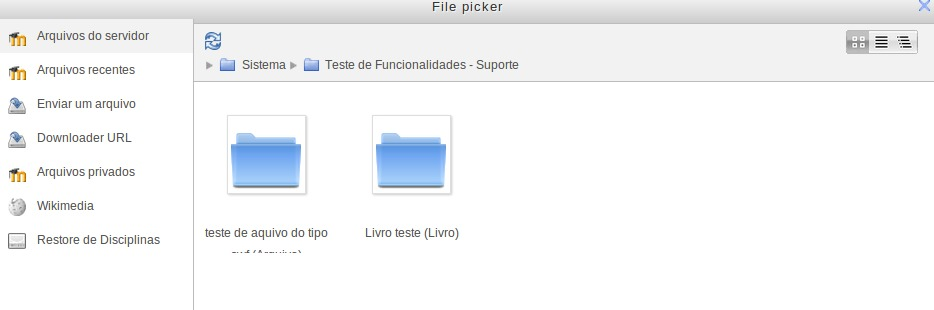
\includegraphics[width=0.5\textwidth]{imagem/cap4/fig30.jpg}}
         \end{center}

\item Navegar entre os diretórios e clicar no arquivo desejado;
\item Se necessário, preencher os campos \textbf{Salvar como}, \textbf{Autor} e selecionar o tipo de licença do arquivo, conforme a Figura abaixo:

         \begin{center}
         \fbox{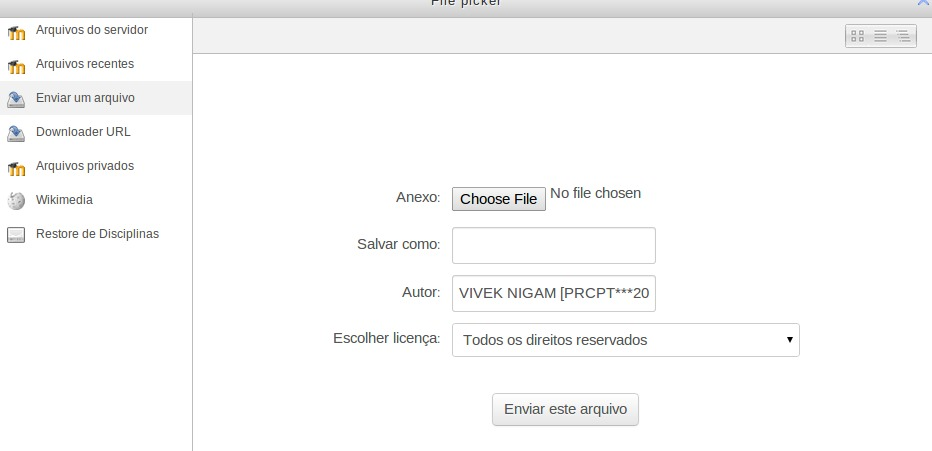
\includegraphics[width=0.5\textwidth]{imagem/cap4/fig31.jpg}}
         \end{center}

\item Clicar em \textbf{Selecione este arquivo}.
\end{enumerate}

Para enviar um arquivo da disciplina:
\begin{enumerate}
\item Na janela exibida, clicar em \textbf{Enviar um arquivo} e seguir os mesmos passos descritos no recurso Pasta (\textbf{Enviando arquivo para uma pasta});
\item Em \textbf{Exibir}, selecionar a opção mais adequada para exibição do arquivo evidenciado para os usuários:
\begin{itemize}
\item \textbf{Automático} - A melhor opção de exibição para o tipo de arquivo é selecionado automaticamente;
\item \textbf{Embed} - O arquivo é exibido dentro da página, abaixo da barra de navegação em conjunto coma descrição do arquivo e todos os blocos;
\item \textbf{Forçar o download} - O usuário é solicitado a baixar o arquivo;
\item \textbf{Abrir} - Apenas o arquivo é exibido na janela do navegador;
\item \textbf{Em uma janela pop-up} - O arquivo é exibido em uma nova janela do navegador sem menus ou uma barra de endereços.
\end{itemize}
\item Caso seja escolhida as opções \textbf{Automático} ou \textbf{Embed}, marcar as caixas de seleção \textbf{Exibir o nome do recurso} ou \textbf{Exibir a descrição do recurso}, se necessário;
\item No caso da escolha da opção \textbf{Em uma janela pop-up}, preencher opcionalmente os campos\textbf{ Largura da janela pop-up}  e \textbf{Altura da janela pop-up} em unidades de pixel.\footnote{Unidade que representa o menor elemento num dispositivo de exibição.}.
\item Na opção\textbf{ Visível}, informar se o recurso ficará disponível ou oculto para os alunos;
\item Caso necessário, preencher o campo \textbf{Número de identificação do módul}o para fins de cálculo de avaliação.
\item Salvar as configurações realizadas clicando no botão \textbf{Salvar e voltar ao curso};
\item Para salvar e retornar para a disciplina ou no botão  \textbf{Salvar e mostrar} para salvar e mostrar o recurso criado.
\end{enumerate}

\section{Rótulo}
Rótulos são utilizados para organizar a parte central de uma disciplina. Com o rótulo é possível inserir todo tipo de informação, em virtude do uso da linguagem HTML. O uso excessivo de rótulos implica no uso demasiado de informação na parte central da disciplina, podendo ocasionar confusão por parte dos alunos.
Rótulos podem ser utilizados para organizar sessões, semanas, tópicos e a divisão das partes de um curso.

\subsection{Acrescentando um rótulo}
Para inserir um rótulo, deve-se:

\begin{enumerate}
\item Na disciplina desejada, clicar no botão \textbf{Ativar Edição} ;
\item Primeiro deve-se clicar na opção \textbf{Adicionar uma atividade ou recurso}, e só então que aparecerá a opção de \textbf{Acrescentar}. Em seguida basta escolher a opção \textbf{Rótulo} na lista \textbf{Recursos} e clicar em \textbf{Acrescentar};
\item No formulário apresentado, preencher obrigatoriamente o campo \textbf{Texto do rótulo}. Neste campo deve-se inserir o texto, imagem e toda informação relativa ao rótulo;
\item Na opção \textbf{Visível}, selecionar se o rótulo deverá ficar oculto ou não para os participantes da disciplina;
\item Salvar as configurações realizadas clicando no botão \textbf{Salvar e voltar ao curso} para salvar e retornar para a disciplina.
\end{enumerate}

\section{URL}

No Moodle. o recurso URL (Uniform Resource Locator)\footnote{Endereço de um recurso (arquivo, impressora etc.), disponível em uma rede; seja a Internet, ou uma rede corporativa}, refere-se a um localizador, ou link, para um sítio ou recurso na Internet. Seu uso é frequente e dá abertura para diversas possibilidades.

\subsection{Acrescentando o recurso URL}
Para adicionar o recurso URL, deve-se:
\begin{enumerate}
\item Na disciplina desejada, clicar no botão  \textbf{Ativar edição};
\item Primeiro deve-se clicar na opção \textbf{Adicionar uma atividade ou recurso}, e só então aparecerá a opção de \textbf{Acrescentar}. Em seguida basta escolher a opção \textbf{URL} na lista \textbf{Recursos} e clicar em \textbf{Acrescentar};
\item No formulário apresentado, preencher obrigatoriamente os campos \textbf{Nome} (nome do recurso que ficará visível na plataforma) e \textbf{Descrição} (informações gerais sobre a URL);
\item No campo \textbf{URL Externa}, preencher com o endereço do sítio ou recurso na Internet;
\item Em \textbf{Exibir}, selecionar a opção mais adequada para exibição do arquivo evidenciado para os usuários:
\subitem \textbf{Automático} - A melhor opção de exibição para o tipo de arquivo é selecionado automaticamente;
\subitem \textbf{Embed} - O arquivo é exibido dentro da página, abaixo da barra de navegação em conjunto coma descrição do arquivo e todos os blocos;
\subitem \textbf{Abrir} - Apenas o arquivo é exibido na janela do navegador;
\subitem \textbf{Em uma janela pop-up} - O arquivo é exibido em uma nova janela do navegador sem menus ou uma barra de endereços.
\item Caso seja escolhida as opções \textbf{Automático} ou \textbf{Embed}, marcar as caixas de seleção \textbf{Exibir o nome da URL} ou \textbf{Exibir a descrição da URL}, se necessário;
\item Na opção \textbf{Visível}, informar se o recurso ficará disponível ou oculto para os alunos;
\item Caso necessário, preencher o campo \textbf{Número de identificação do módulo} para fins de cálculo de avaliação.
\item Salvar as configurações realizadas clicando no botão \textbf{Salvar e voltar ao curso}  para salvar e retornar para a disciplina ou no botão \textbf{Salvar e mostrar}  para salvar e mostrar o recurso criado.
\end{enumerate}

\section{Livro}
Para criar um recurso Livro, antes de mais nada, é necessário \textbf{Ativar a Edição} na página da disciplina.
Na semana escolhida, deve-se clicar na opção \textbf{Adicionar uma atividade ou recurso}, e só então aparecerá a opção de \textbf{Acrescentar}. Daí basta escolher a opção \textbf{Livro} na lista \textbf{Recursos} e clicar em \textbf{Acrescentar}; (Veja a Figural \ref{fig:cap4_32}).
\begin{figure}[htbp]
         \begin{center}
         \fbox{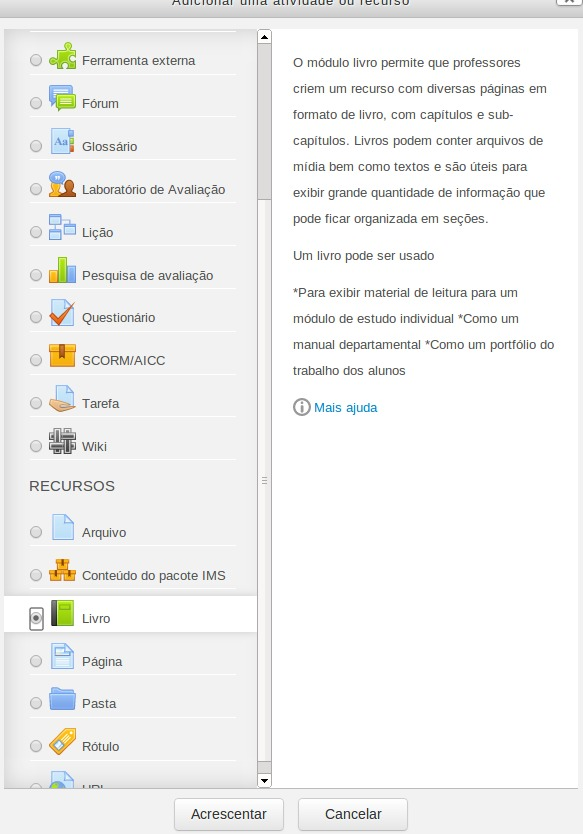
\includegraphics[width=0.5\textwidth]{imagem/cap4/fig32.jpg}}
          \caption{Acrescentando Livro}
          \label{fig:cap4_32}
         \end{center}
\end{figure}

Abrirá uma página para a configuração do Livro. Nela você encontrará os seguintes campos e opções:

\begin{table}[htbp]
\begin{flushleft}
    \begin{tabular}{p{6cm}|p{9cm}} \hline
\rowcolor[rgb]{0.8,0.8,0.8} \textbf{GERAL}&\\\hline
\textbf{Nome} & Escreve-se o nome do livro, que aparecerá no link do recurso, na página da disciplina. \\\hline
\textbf{Descrição} & Uma breve descrição do livro. \\\hline
\textbf{Formatação} & A forma como os capítulos aparecerão no índice. As principais são Números e Bolinhas \\\hline
\textbf{Títulos Personalizados}& Os títulos dos capítulos são mostrados automaticamente apenas no sumário, permitindo que se personalize os títulos no conteúdo do capítulo, se este não for selecionado os títulos dos capítulos serão inseridos automaticamente no topo da página de conteúdo. \\\hline
\rowcolor[rgb]{0.8,0.8,0.8} \textbf{CONFIGURAÇÕES COMUNS DE MÓDULOS}&\\\hline
\textbf{Visíveis} & Mostrar ou Ocultar o recurso na página da disciplina. \\\hline
\textbf{Número de Identificação} & O Número ID identifica a atividade para fins de cálculo de avaliação. Se a atividade não estiver inclusa em nenhum cálculo de avaliação então o campo do Número ID pode ser deixado em branco.
O Número ID também pode ser definido na página de edição do cálculo das notas no Relatório de Avaliação, embora ele só possa ser editado na página de atualização da atividade. \\\hline
\end{tabular}
%   \label{tab:ConfDisciplina}
  \end{flushleft}
\end{table}%
Ao final além do botão Cancelar, existem botões para Salvar e voltar para o curso, e Salvar e Mostrar. Ao clicar no primeiro o livro é criado e volta para a página da disciplina. Se clicar no livro, abre então a configuração do primeiro capítulo (para o professor). Se optar-se por clicar no segundo, abre diretamente na configuração do primeiro capítulo.

O uso da palavra capítulo repete o que é usado no Moodle (Veja a Figura \ref{fig:cap4_33}), porém o livro é um conjunto de índice (uma lista dos itens disposta em coluna vertical, no lado esquerdo da página) e conteúdos (ao clicar em cada item abre o conteúdo relacionado).

\begin{figure}[htbp]
         \begin{center}
         \fbox{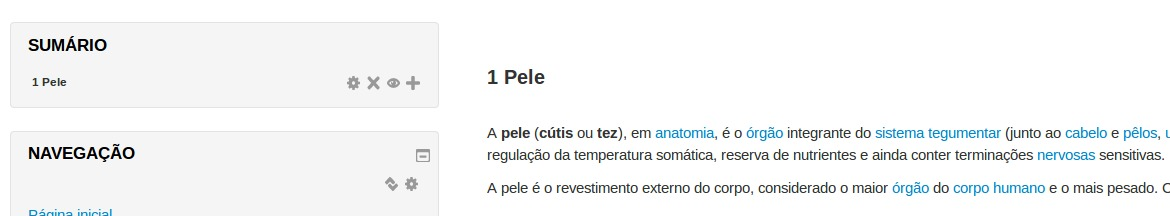
\includegraphics[width=0.7\textwidth]{imagem/cap4/fig33.jpg}}
          \caption{Visualização de capítulos}
          \label{fig:cap4_33}
         \end{center}
\end{figure}

Ao Ativar Edição no livro, cada item do índice ganha o tradicional menu de ícones para edição do Moodle. Relembrando rapidamente, as setas permitem mover o item, a mão abre a edição do mesmo, o X exclui, o olho oculta ou torna visível e, finalmente, o ícone exclusivo do livro, que cria um novo capítulo (item) abaixo do item escolhido.

Ao criar um capítulo as seguintes configurações estarão disponíveis no canto superior esquerdo do sítio do Moodle (Veja a Figura \ref{fig:cap4_34}, e a Tabela \ref{tab:ConfCaptulo}):
\begin{figure}[htbp]
         \begin{center}
         \fbox{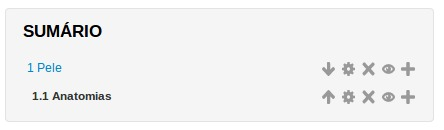
\includegraphics[width=0.4\textwidth]{imagem/cap4/fig34.jpg}}
          \caption{Opções de Edição de Capítulo}
          \label{fig:cap4_34}
         \end{center}
\end{figure}
\begin{table}[htbp]
\begin{flushleft}
    \begin{tabular}{p{6cm}|p{9cm}} \hline
\rowcolor[rgb]{0.8,0.8,0.8} \textbf{EDITAR}&\\\hline
\textbf{Título de capítulo} & O título do capítulo, que aparecerá no índice e no topo do conteúdo, caso a opção de Título Personalizado não tiver sido marcada na criação do livro. \\\hline
\textbf{Sub-capítulo} & Uma caixa de seleção que marcada fará com que o capítulo se torne um sub-capítulo do imediatamente anterior no índice.\\\hline
\textbf{Conteúdo} & O texto do capítulo.\\\hline

\end{tabular}
    \caption{Detalhamento das opções de edição de capítulo}
  \label{tab:ConfCaptulo}
  \end{flushleft}
\end{table}%
